\section{Специальный регулятор}

Рассмотрим замкнутую системы с объектом управления, описываемым передаточной функцией:
\begin{equation}
    W(s) = \frac{3}{s^2 + 7.5s + 2}
\end{equation}
И регулятором, описываемым передаточной функцией:
\begin{equation}
    H(s) = \frac{\sum_{k=0}^{m}(b_ks^k)}{\sum_{k=0}^{n}(a_ks^k)}
\end{equation}
Найдем образ Лапласа входного сигнала:
\begin{equation}
    U(s) = L\{4 \sin(0.25 t)\} = \frac{1}{s^2 + 0.25^2}
\end{equation}
Исходя из числителя образа Лапласа входного сигнала, можно предположить, что передаточная функция регулятора будет иметь вид:
\begin{equation}
    H(s) = \frac{k_2s^2 + k_1s + k_0}{s^2 + 0.25^2}
\end{equation}
Найдем образ ошибки согласно формуле:
\begin{multline}
    E = \frac{D_wD_h}{D_wD_h + N_wN_h} \cdot \frac{N_u}{D_u} = \frac{(s^2 + 7.5s + 2)(s^2 + 0.25^2)}{(s^2 + 7.5s + 2)(s^2 + 0.25^2) + 3(k_2s^2 + k_1s + k_0)} \cdot \frac{1}{s^2 + 0.25^2} =  \\
    \frac{(s^2 + 7.5s + 2)}{(s^2 + 7.5s + 2)(s^2 + 0.25^2) + 3(k_2s^2 + k_1s + k_0)}  = \\
    \frac{s^2 + 7.5s + 2}{s^4 + 7.5s^3 + (3k_2 + 0.25^2 + 2)s^2 + (7.5 \cdot 0.25^2 + 3k_1)s + 2 \cdot 0.25^2 + 3k_0}
\end{multline}
Подходящими значениями коэффициентов регулятора будут:
\begin{equation}
    k_2 = 2, k_1 = 2, k_0 = 1
\end{equation}
при них система будет устойчива, согласно критерию Гурвица для система 4 порядка. Промоделируем систему, представленную на рис. \ref{fig:task6_scheme}.

Теоретическое значение установившегося значения ошибки равно:
\begin{equation}
    e_{\text{set}} = \lim_{s \to 0} sE = \frac{0}{2 + 0.25^2 + 3k_0} = 0
\end{equation}
\begin{figure}[ht!]
    \centering
    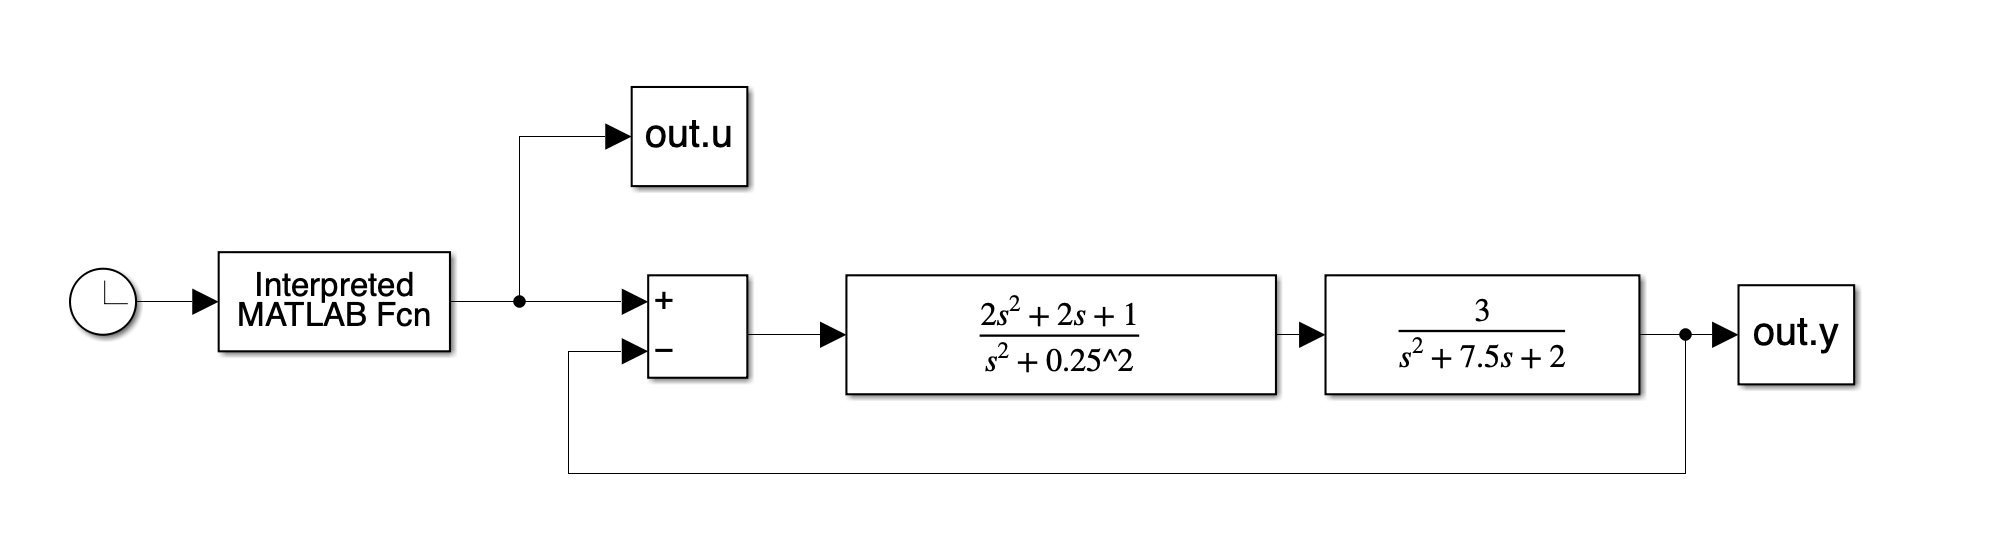
\includegraphics[width=\textwidth]{"media/scheme6.png"}
    \caption{Схема моделирования системы}
    \label{fig:task6_scheme}
\end{figure}
Результаты моделирования приведены на рис. \ref{fig:task6_out} и \ref{fig:task6_error}.
\begin{figure}[ht!]
    \centering
    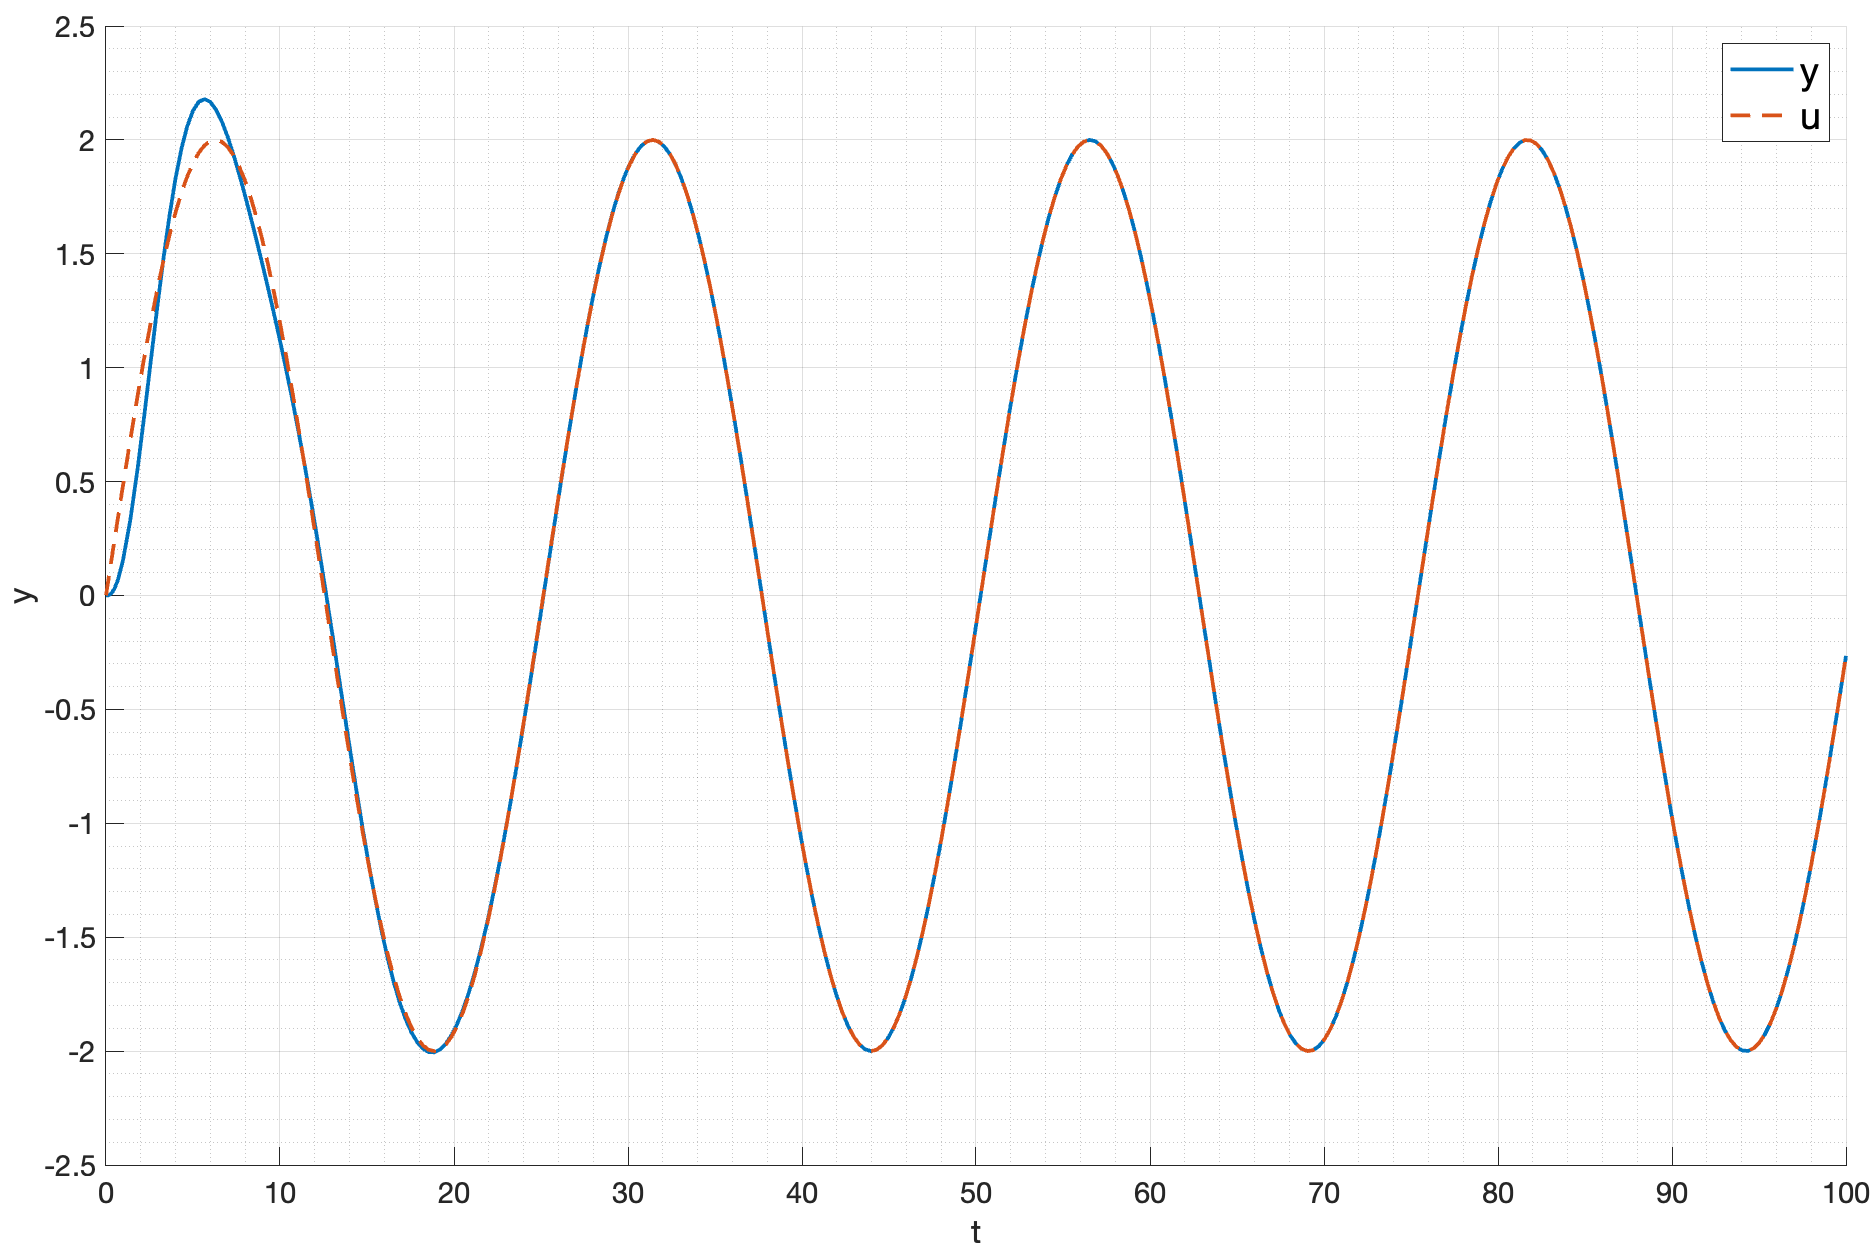
\includegraphics[width=\textwidth]{media/plots/task6_out.png}
    \caption{График выходного сигнала}
    \label{fig:task6_out}
\end{figure}
\begin{figure}
    \centering
    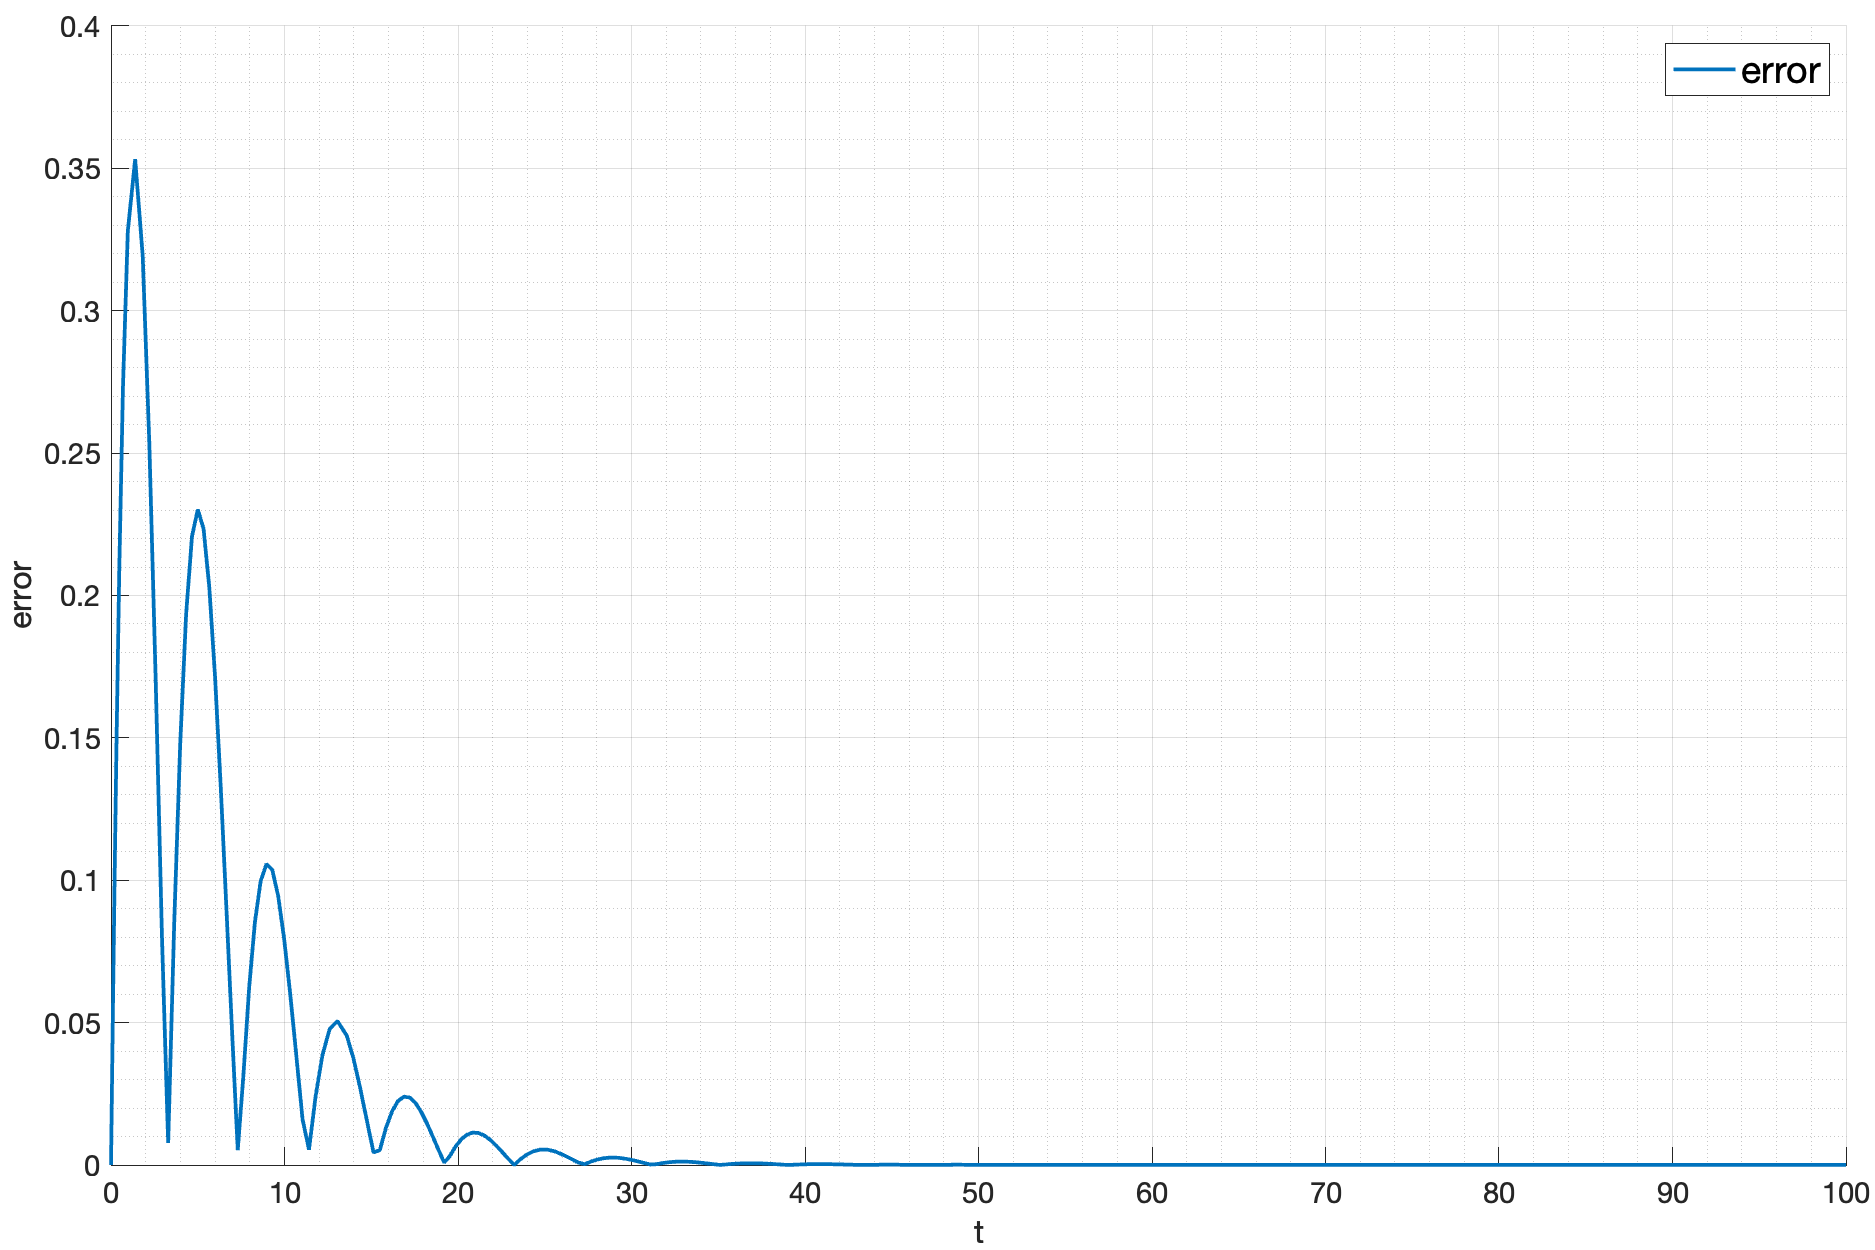
\includegraphics[width=\textwidth]{media/plots/task6_error.png}
    \caption{График ошибки}
    \label{fig:task6_error}
\end{figure}
Видно, что система в точности повторяет входной сигнал после некоторого времени, ошибка
стремится к нулю, что соответствует теоретическим расчетам.

\subsection{Вывод}
В данном пункте была рассмотрена система со специальным регулятором, который позволяет
получить систему с нулевой установившейся ошибкой. 